\documentclass{article}%
\usepackage[T1]{fontenc}%
\usepackage[utf8]{inputenc}%
\usepackage{lmodern}%
\usepackage{textcomp}%
\usepackage{lastpage}%
\usepackage[head=40pt,margin=0.5in,bottom=0.6in]{geometry}%
\usepackage{graphicx}%
%
\title{\textbf{Docentes protestaron en Mérida para exigir mejoras salariales}}%
\author{El Nacional Web}%
\date{23/11/2018}%
%
\begin{document}%
\normalsize%
\maketitle%
\textbf{URL: }%
http://www.el{-}nacional.com/noticias/protestas/docentes{-}protestaron{-}merida{-}para{-}exigir{-}mejoras{-}salariales\_260852\newline%
%
\textbf{Periodico: }%
EN, %
ID: %
260852, %
Seccion: %
Protestas\newline%
%
\textbf{Palabras Claves: }%
Mérida, Protestas, Sociedad\newline%
%
\textbf{Derecho: }%
2.3, %
Otros Derechos: %
, %
Sub Derechos: %
2.3.4\newline%
%
\textbf{EP: }%
SI\newline%
\newline%
%
\textbf{\textit{Un grupo de personas impidió por más de dos horas el paso de los vehículos}}%
\newline%
\newline%
%
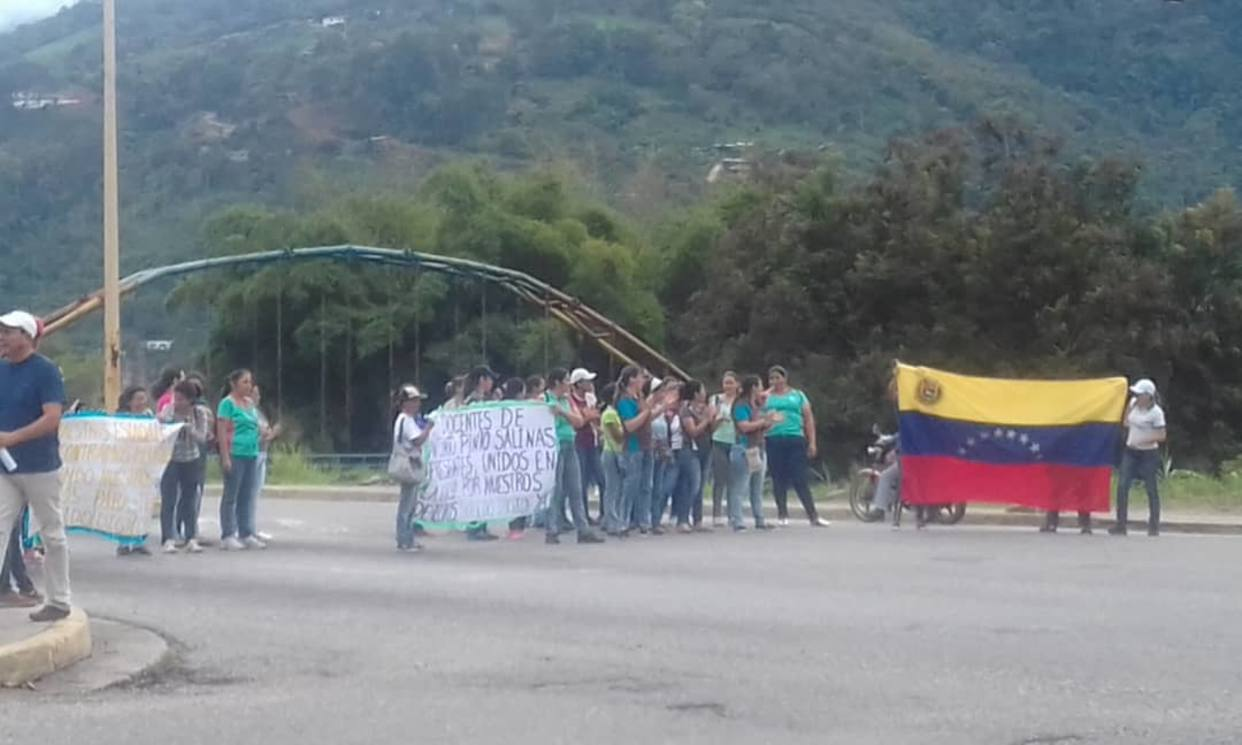
\includegraphics[width=300px]{144.jpg}%
\newline%
%
Un grupo de docentes adscritos a la Gobernación del estado Mérida realizan una protestaron este viernes para exigir mejoras salariales.%
\newline%
%
Leonardo León, ~corresponsal de~El Nacional~en la entidad, explicó vía Twitter que las personas se encuentran en una avenida de la parroquia Santa Cruz de Mora.%
\newline%
%
En la imagen difundida por el periodista se puede observar cómo los docentes cerraron la vía para impedir el paso de los vehículos. Las personas sostienen banderas y carteles con mensajes alusivos a su protesta.%
\newline%
%
\end{document}